\textbf{{1.内存管理的功能}}

\textbf{a.~}{内存的分配和回收;}

\textbf{b.} 地址变换;

\textbf{c.} 扩充内存;

\textbf{d.} 存储保护。

\textbf{{2.应用程序的编译、链接与装入}}

\textbf{a.} {从源程序到执行的进程,经历了编译、链接、装入3个步骤;}

\textbf{b.}
地址转换将逻辑地址转换为物理地址,这个过程叫做\textbf{重定位}。不同地址的变换过程如下图所示。

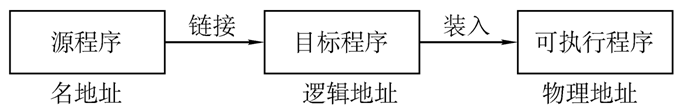
\includegraphics[width=3.12500in,height=0.50000in]{png-jpeg-pics/0862581A20AADD62F49C0B16737DE24C.png}

\textbf{c.}
程序的链接有3种方式:静态链接、运行时动态链接、装入时动态链接;\\
\textbf{d.~}程序的装入也有3种方式:绝对装入、可重定位装入、动态运行装入。

{\textbf{3. 物理地址和逻辑地址}}

\textbf{a.}
{逻辑地址是指由程序产生的与段(与页无关,因为只有段对用户可见)相关的偏移地址部分。}

\textbf{b.}
物理地址是指出现在CPU外部地址总线上的寻址物理内存的地址信号,是逻辑地址变换后的最终结果地址,物理地址空间是指内存中物理地址单元的集合。

\textbf{{4.内存保护}}

内存保护是为了防止一个作业有意或无意地破坏操作系统或其他作业。常用的存储保护方法有界限寄存器方法和存储保护键方法。\\
\textbf{a.
界限寄存器方法:}有两种,分别是上、下界寄存器方法和基址和限长寄存器方法。上、下界寄存器方法\textbf{{采用上、下界寄存器分别存放作业的结束地址和开始地址}}。在作业运行过程中,将每一个访问内存的地址都同这两个寄存器内容进行比较,如超出范围便产生保护性中断;{基址和限长寄存器方法}{\textbf{采用基}}{\textbf{{址和限长寄存器分别存放作业的起始地址及作业的地址空间长度}}。当作业执行时,将每一个访问内存的相对地址和现场寄存器比较,如果超过了限长寄存器的值,则发出越界中断信号,并停止作业的运行。}

\textbf{b.
存储保护键方法:}存储保护键方法是\textbf{给每个存储块分配一个单独的保护键},它相当于一把``锁''。此外,\textbf{进入系统的每个作业也被赋予一个保护键},它相当于一把``钥匙''。当作业运行时,检查``钥匙''和``锁''是否匹配,如果二者不匹配,则系统发出保护性中断信号,停止作业运行。
